\chapter{Software Engineering Process}

As the majority of the work put into this project was in developing the software artifact, I was focused from the beginning on following an effective software engineering process.

\section{Process}
I employed an agile\cite{Agile} methodology throughout my work on this project. 

One of the key Agile principles is to `Deliver working software frequently'\cite{AgileKey}. I followed this from the beginning by setting myself intermediary deadlines, by which I planned to demo working sections of project. These deadlines were discussed and agreed upon with my supervisor. This helped me stay focused on getting the features I needed working while avoiding premature optimisation.

Another primary principle of the Agile Manifesto is to `Welcome changing requirements, even late in development'\cite{AgileKey}. As an example of this, one of my original requirements involved assessing how accurately my software could gather people's real world views. After thinking more about the psychological aspects of this question, my supervisor and I decided that this would be too difficult, and would be closer to psychology than computer science. After realising this, we changed this requirement to performing a comparatively simple user evaluation. 

\section{Tools}
With this in mind, one of the first tools I employed was Git\cite{Git}.
Considering the length of the project, it was reasonable to suspect that there may come a time when I would have to revert my project to a previous point if something was broken.
Version control software was the obvious solution, and Git is the one of these that I have the most experience with. To complement this, I set up a master GitHub\cite{GitHub} repository to use as a backup.

In addition to serving as a backup, GitHub provides a useful set of project tracking features. 
I did consider other tools often used to track projects, such as Trello\cite{Trello}, but in the end decided that GitHub's ability to reference aspects of the code (thanks to them being stored in the same place) made it better suited for my needs. 
Here I will outline the features that I used and describe how they helped my development process:

\paragraph{Issues} These are a core element of GitHub; any task that needs completing is documented as an issue.
I kept my issues fairly high-level, as I have found previously that too much detail in issues results in spending excessive amounts of time managing them or some inevitably become outdated. Figure \ref{fig:issue} shows an example issue.

\begin{figure}[!h]
	\centering
	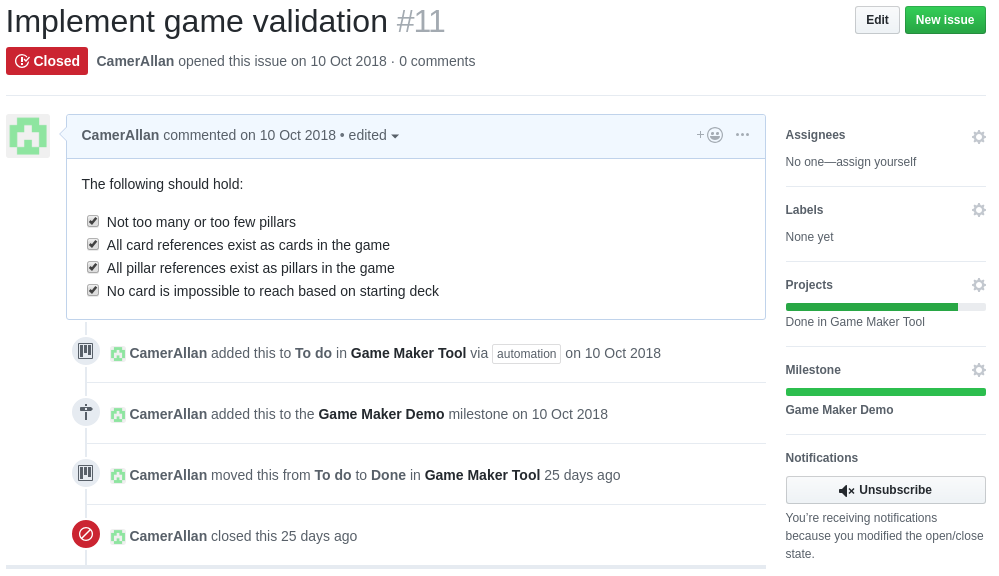
\includegraphics[width=0.9\textwidth]{./images/softeng/issue.png}
	\caption{An example of an issue, note the assigned description, project, and milestone.}
	\label{fig:issue}
\end{figure}

\paragraph{Projects} Issues alone can become unorganised, so I made use of GitHub's projects feature. 
I split my work into four parts - game, game maker, visualisation and backend then made a project for each of these. 
This allowed me to keep issues relating to different parts of the project separate, making it easier to focus on one section at a time.

\begin{figure}[!h]
	\centering
	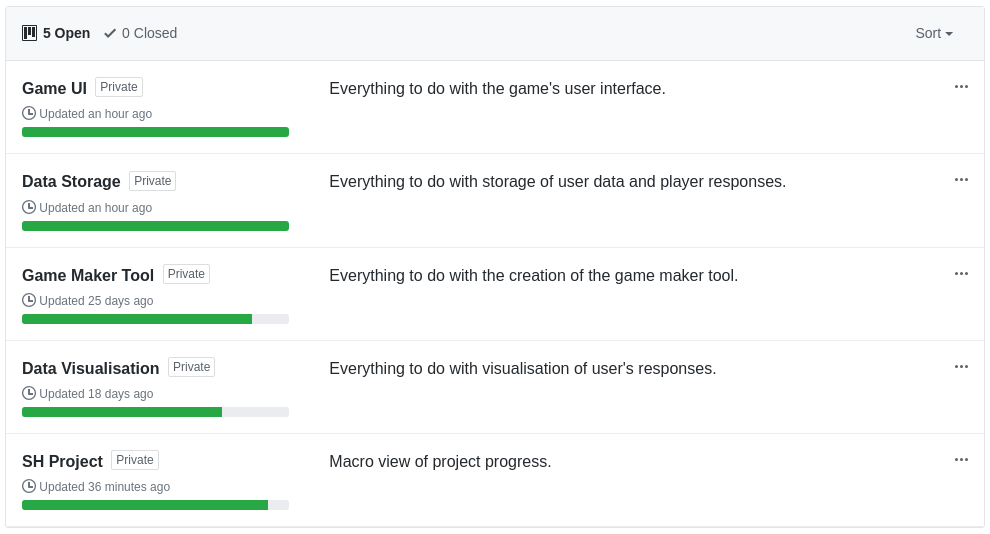
\includegraphics[width=0.9\textwidth]{./images/softeng/projects.png}
	\caption{Project overview page.}
	\label{fig:projects}
\end{figure}

Each project has its own kanban-style\cite{KBAN} board, used to track its progress, an example of which can be seen in figure \ref{fig:board}. Issues assigned to a project start in the \c{todo} column. When being worked on, I would move them into \c{In progress}, and finally when closed they are automatically moved to \c{Done}.

The project overview visualises the proportion of issues in each column, providing an instant, accurate depiction of progress.

\begin{figure}[!h]
	\centering
	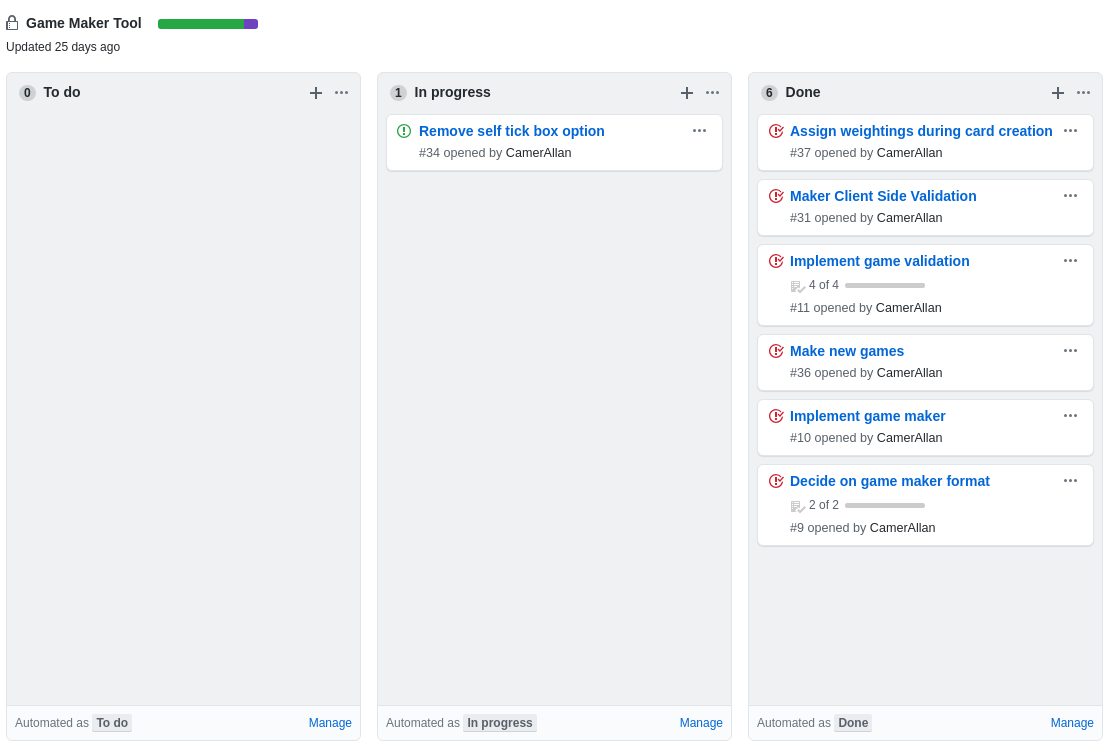
\includegraphics[width=0.9\textwidth]{./images/softeng/board.png}
	\caption{Example project board towards the end of the project.}
	\label{fig:board}
\end{figure}

\paragraph{Milestones} The first step I took in tracking my project was to set my Milestones. These are an aspect of a GitHub project that serve as a deadline, to which issues can be added. 
Completing and closing these issues then automatically provides a visualisation of progress towards a milestone, as can be seen in figures \ref{fig:closed_milestones} and \ref{fig:open_milestones}. 
These made for a helpful overview, which was useful both for myself, and for sharing my progress with my supervisor.

I decided on these milestones early on by estimating the dates by which I could complete core parts of the project. As this was done in advance I was not able to be precise with demo dates, however I completed the vast majority of work for each milestone in advance of the deadline, so I consider this a successful element of my planning.

\begin{figure}[!h]
	\centering
	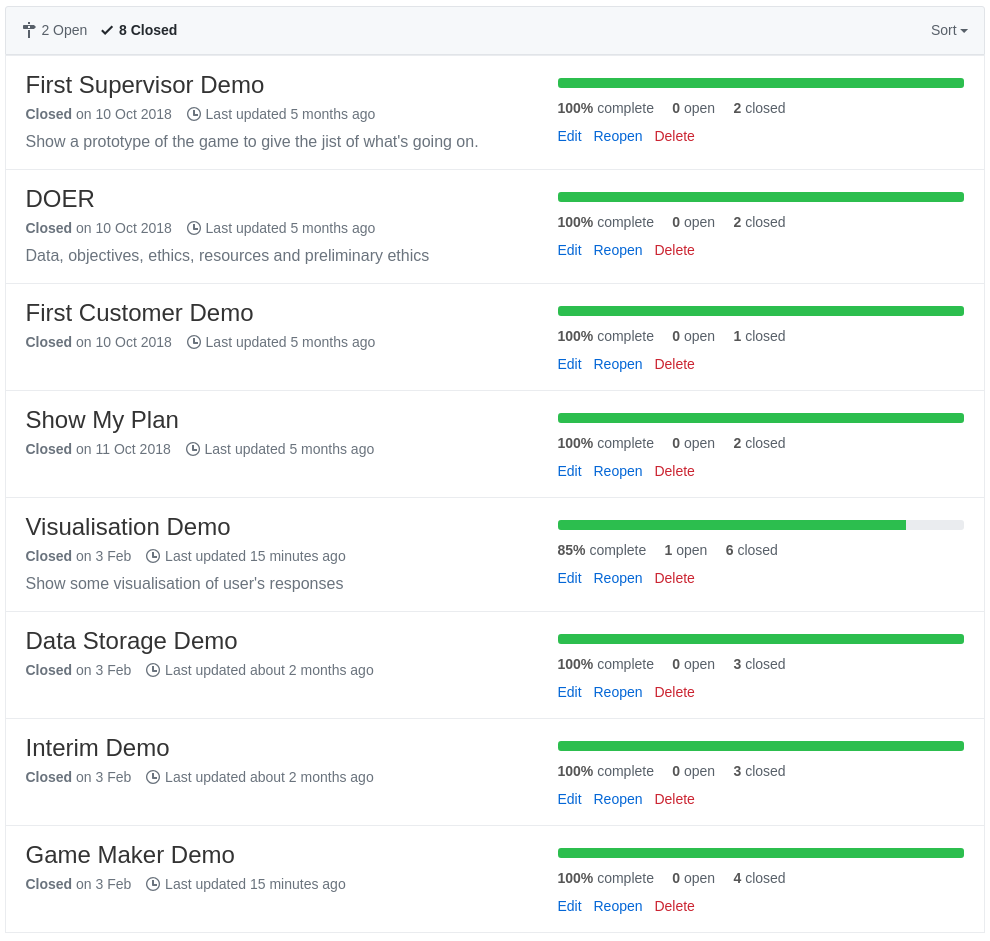
\includegraphics[width=0.9\textwidth]{./images/softeng/closed_milestones.png}
	\caption{Closed (completed) milestones towards the end of the project}
	\label{fig:closed_milestones}
\end{figure}

\begin{figure}[!h]
	\centering
	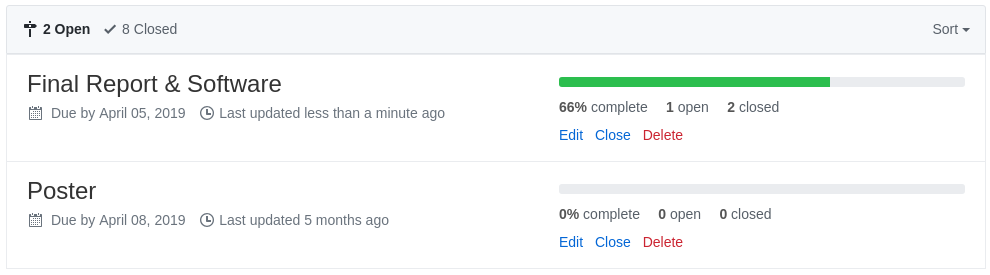
\includegraphics[width=0.9\textwidth]{./images/softeng/open_milestones.png}
	\caption{Open milestones towards the end of the project}
	\label{fig:open_milestones}
\end{figure}

